\section{Numerical results} \label{sec:res}
Let us now discuss the performance of the symplectic model reduction with a weighted inner product. In \cref{sec:res.1,sec:res.1.1} we apply the model reduction to equations of a vibrating elastic beam without and with cavity, respectively. And we examine the evaluation of the nonlinear terms in the model reduction of the sine-Gordon equation, in section \cref{sec:res.2}.

\subsection{The elastic beam equation} \label{sec:res.1}
Consider the equations governing small deformations of a clamped elastic body $\Gamma\subset \mathbb R^{3}$ as 
\begin{equation} \label{eq:res.1}
\left\{
\begin{aligned}
	u_{tt}(t,x) &= \nabla \cdot \sigma + f, \quad & x\in \Gamma, \\
	u(0,x) &= \vec 0, & x\in \Gamma,\\
	\sigma \cdot n &= \tau, & x \in \partial \Gamma_\tau,\\
	u(t,x) &= \vec 0, & x \in\partial \Gamma \backslash \partial \Gamma_\tau,
\end{aligned}
\right.
\end{equation}
and
\begin{equation}  \label{eq:res.2}
	\sigma = \lambda (\nabla \cdot u) I + \mu(\nabla u + (\nabla u)^T).
\end{equation}
Here $u:\Gamma \to \mathbb{R}^3$ is the unknown displacement vector field, subscript $t$ denotes derivative with respect to time, $\sigma:\Gamma \to \mathbb{R}^{3\times 3}$ is the stress tensor, $f$ is the body force per unit volume, $\lambda$ and $\mu$ are Lam\'e's elasticity parameters for the material in $\Gamma$, $I$ is the identity tensor, $n$ is the outward unit normal vector at the boundary and $\tau:\partial \Gamma_\tau \to \mathbb R^3$ is the traction at a subset of the boundary $\partial \Gamma_\tau$ \cite{langtangen2017solving}. We refer to \Cref{fig:0}(a) for a snapshot of the elastic beam.

\begin{figure}[t] \label{fig:0}
\begin{tabular}{cc}
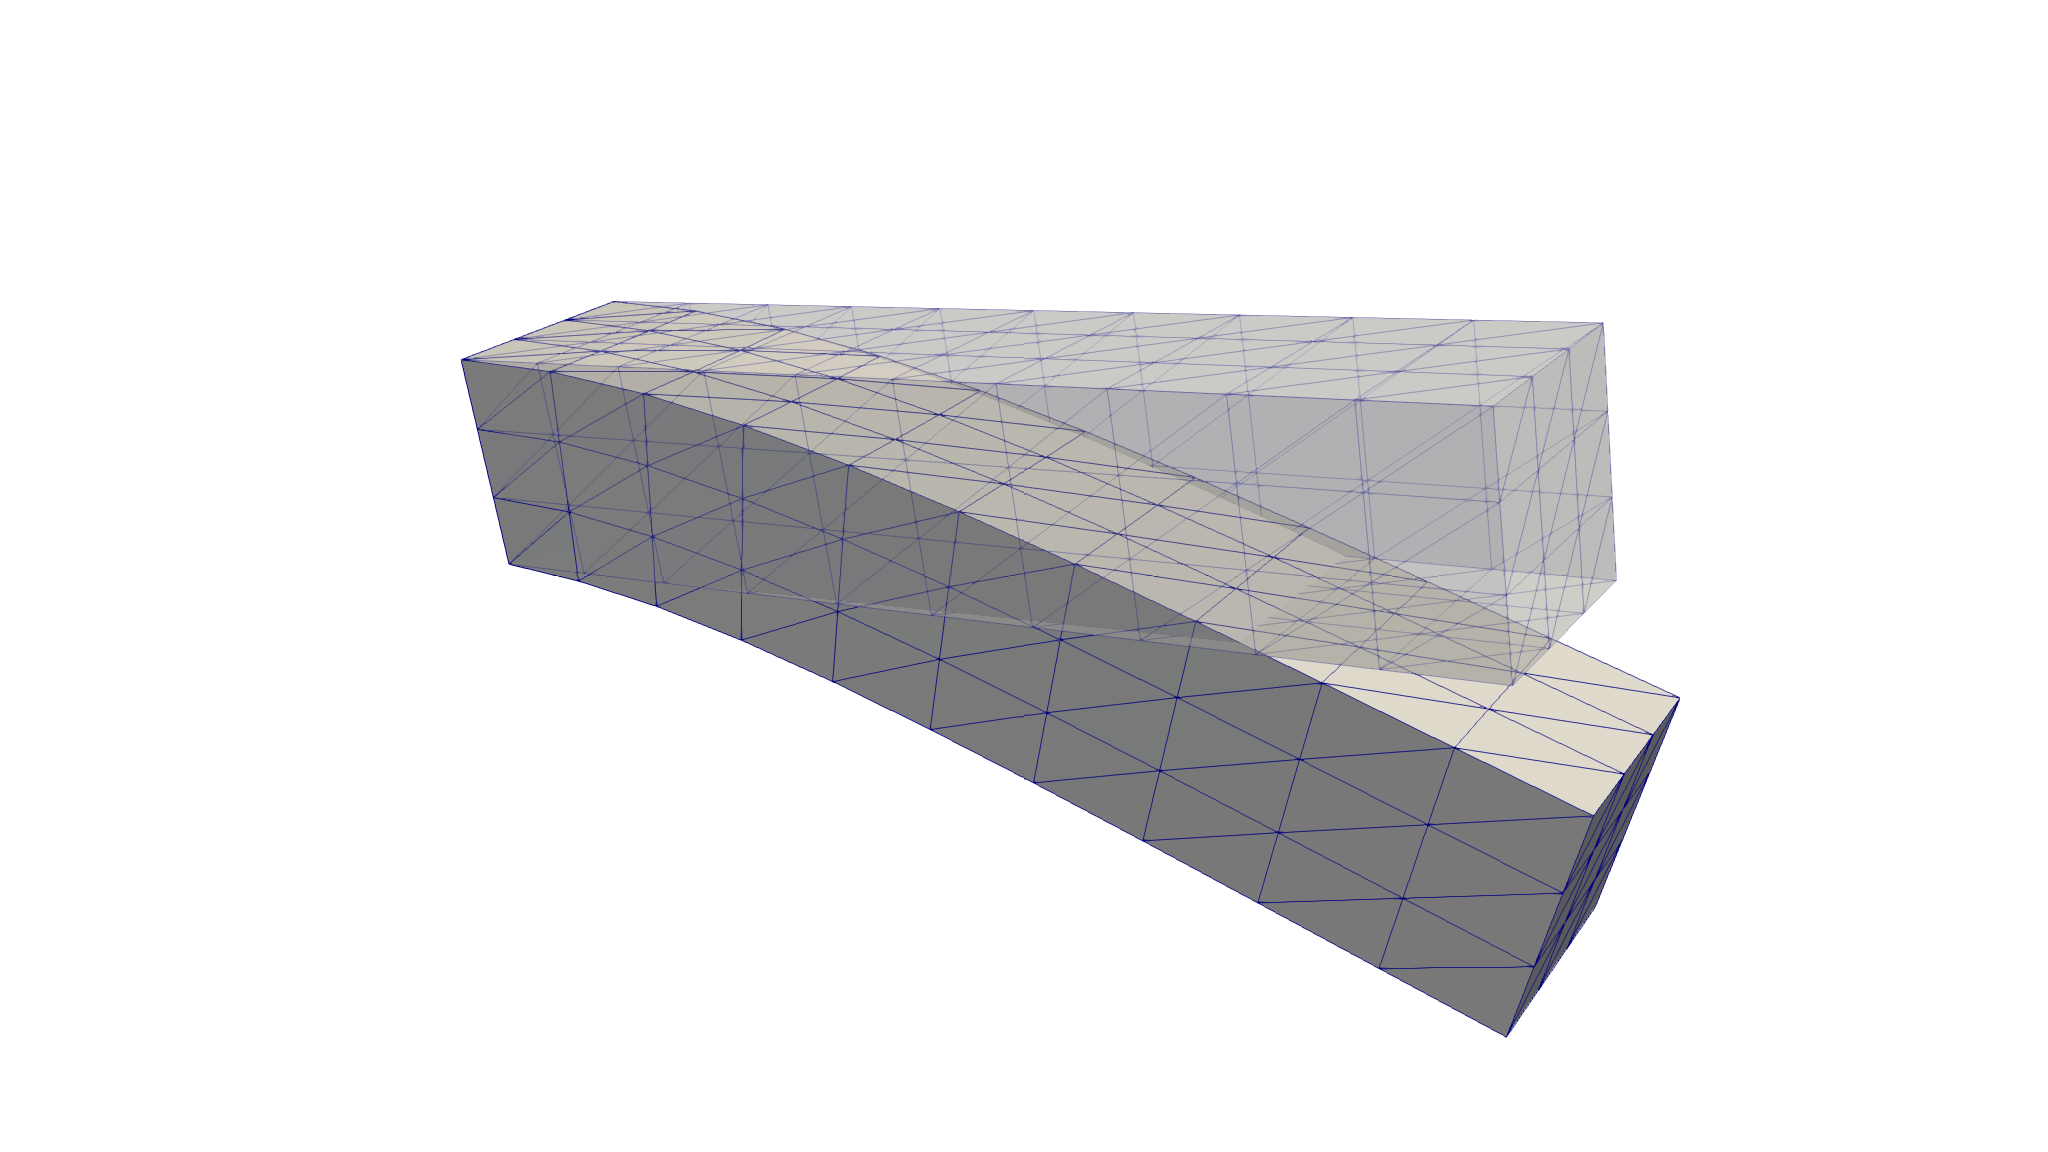
\includegraphics[width=0.45\textwidth]{./figs/beam3d.png} & 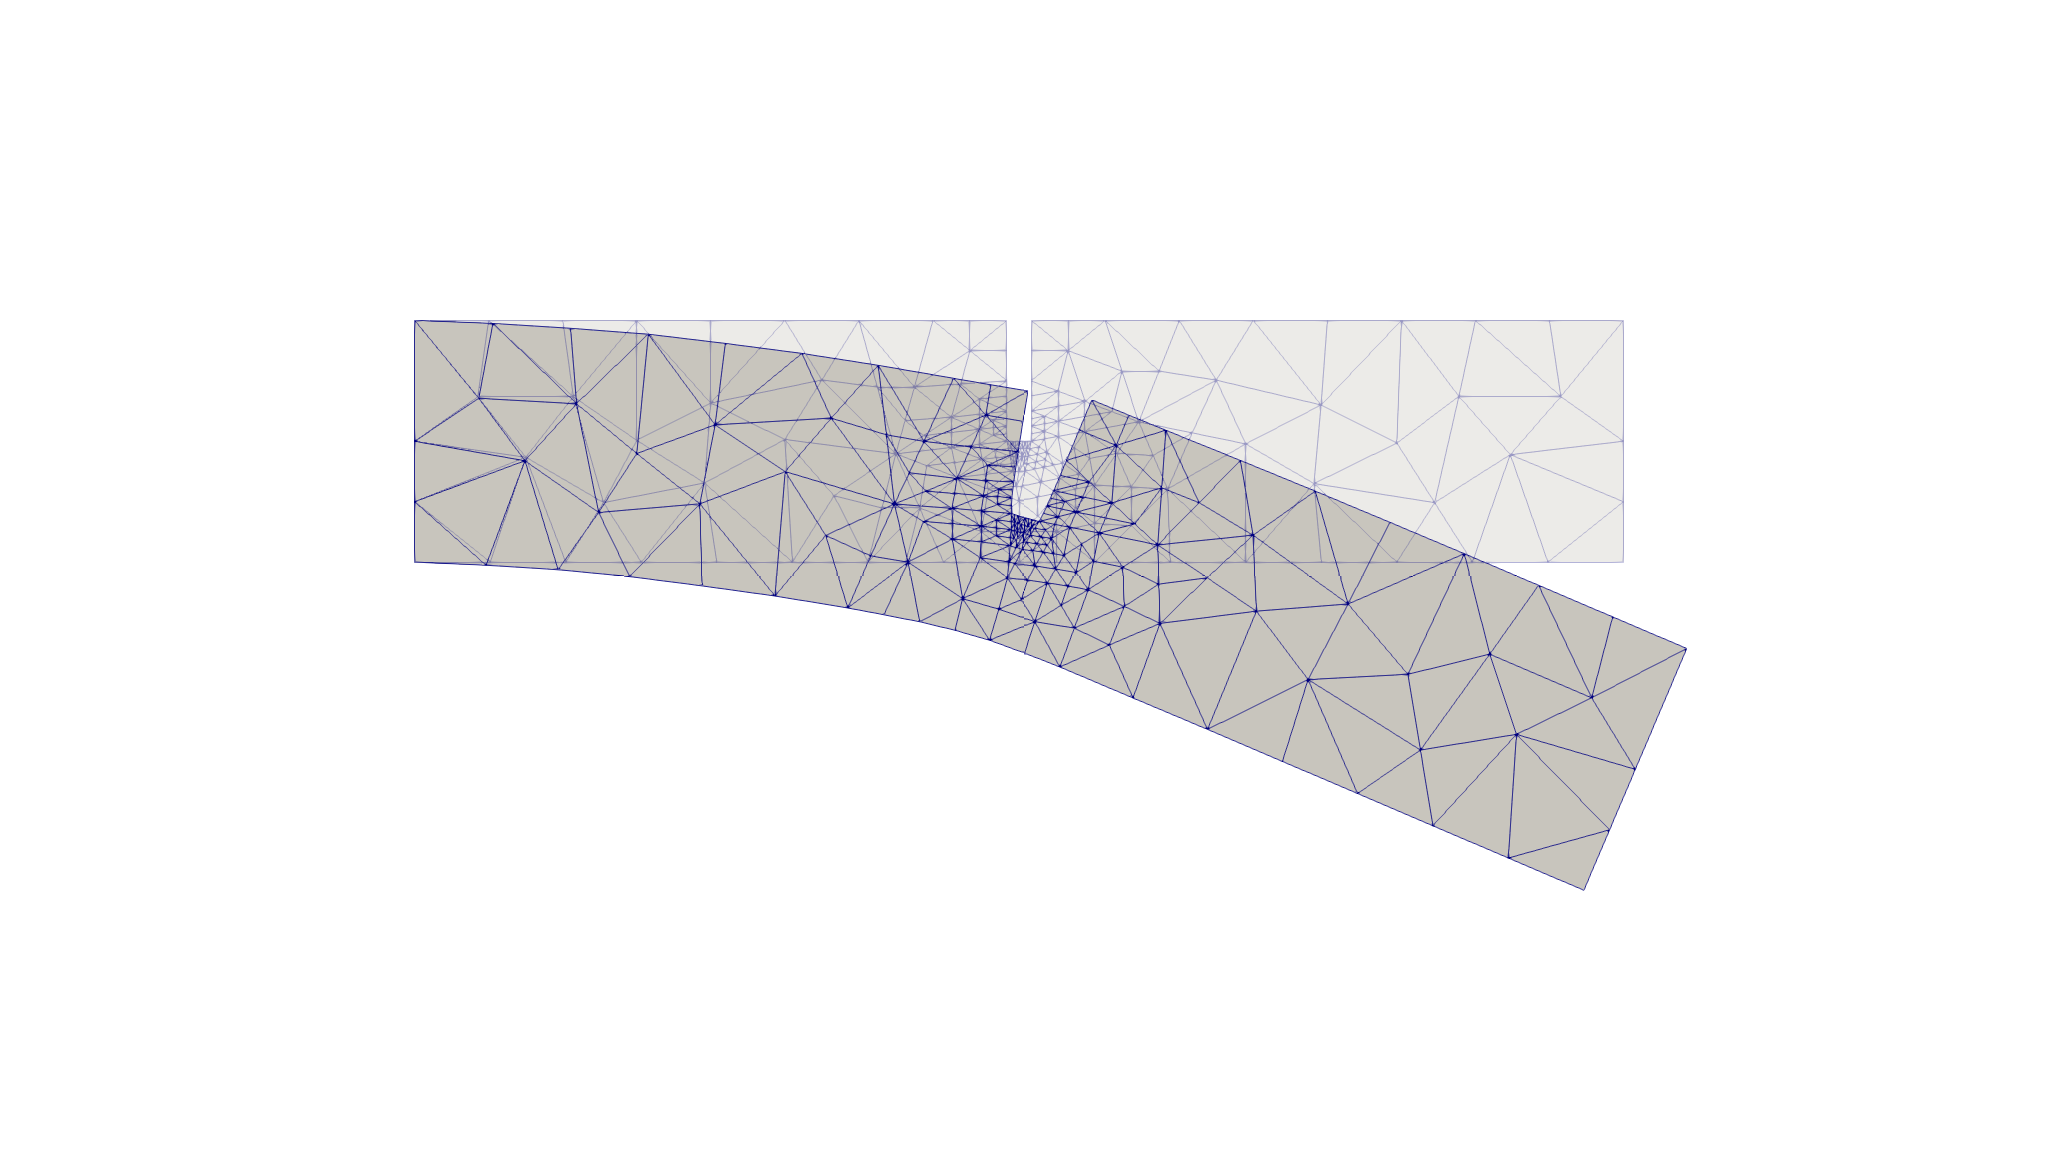
\includegraphics[width=0.45\textwidth]{./figs/beam2d.png} \\
(a) & (b)
\end{tabular}
\caption{(a) initial condition and a snapshot of the 3D beam. (b) initial condition and a snapshot of the 2D beam with cavity. }
\end{figure}

We define a vector valued function space as $V = \{ u \in (L^2(\Gamma))^3 : \| \nabla u_i \|_2 \in L^2 \text{, } i=1,2,3\text{, } u = \vec 0 \text{ on } \partial \Gamma_\tau \}$, equipped with the standard $L^2$ inner product $(\cdot,\cdot):V\times V \to \mathbb R$, and seek the solution to (\ref{eq:res.1}). To derive the weak formulation of (\ref{eq:res.1}), we multiply it with the vector valued test function $v \in V$, integrate over $\Gamma$, and use integration by parts to get 
%\begin{equation}  \label{eq:res.3}
%	\int_{\Gamma} u_{tt} \cdot v\ dx = \int_{\Gamma} (\nabla \cdot \sigma) \cdot v \ dx + \int_{\Gamma} f \cdot v \ dx.
%\end{equation}
%We may integrate the first term on the right hand side by parts to obtain
\begin{equation}  \label{eq:res.4}
	\int_{\Gamma} u_{tt} \cdot v\ dx = - \int_{\Gamma} \sigma : \nabla v \ dx+ \int_{\partial \Gamma_\tau} (\sigma \cdot n) \cdot v\ ds +  \int_{\Gamma} f \cdot v \ dx,
\end{equation}
where $\sigma : \nabla v = \sum_{i,j}\sigma_{ij}(\nabla v)_{ji}$ is the tensor inner product. Note that the skew-symmetric part of $\nabla v$ vanishes over the product $\sigma : \nabla v$, since $\sigma$ is symmetric. By prescribing the boundary conditions to (\ref{eq:res.4}) we recover
\begin{equation} \label{eq:res.5}
	\int_{\Gamma} u_{tt} \cdot v\ dx = - \int_{\Gamma} \sigma : \text{Sym}(\nabla v) \ dx+ \int_{\partial \Gamma_\tau} \tau \cdot v\ ds +  \int_{\Gamma} f \cdot v \ dx,
\end{equation}
with Sym$(\nabla v) = (\nabla v + (\nabla v)^T)/2$. The variational form associated to (\ref{eq:res.1}) is
\begin{equation} \label{eq:res.6}
	(u_{tt},v) = - a(u,v) + b(v), \quad u,v\in V,
\end{equation}
where
\begin{equation} \label{eq:res.7}
\begin{aligned}
	a(u,v) = \int_{\Gamma} \sigma : \text{Sym}(\nabla v) ~ dx, ~
	b(v) = \int_{\partial \Gamma_\tau} \tau \cdot v ~ ds +  \int_{\Gamma} f \cdot v \ dx.
\end{aligned}
\end{equation}
To obtain the FEM discretization of (\ref{eq:res.6}), we triangulate the domain $\Gamma$ and define vector valued piece-wise linear basis functions $\{\phi_i\}_{i=1}^{N_h}$, referred to as the \emph{hat functions}. We define the FEM space $V_h$, an approximation of $V$, as the span of those basis functions. Projecting (\ref{eq:res.6}) onto $V_h$ yields the discretized weak form
\begin{equation} \label{eq:res.8}
	((u_h)_{tt},v_h) = - a(u_h,v_h) + b(v_h),\quad u_h,v_h\in V_h.
\end{equation}
Any particular function $u_h$ can be expressed as $u_h = \sum_{i=1}^{N_h} q_i \phi_i$, where $q_i$, $i=1,\dots,N_h$, are the expansion coefficients. Therefore, by choosing test functions $v_h = \phi_i$, $i=1,\dots,N_h$, we obtain the ODE system
\begin{equation} \label{eq:res.9}
	M\ddot q = -K q + g_{q}.
\end{equation}
where $q=(q_1,\dots,q_{N_h})^T$ are unknowns, the \emph{mass matrix} $M\in \mathbb R^{N_h\times N_h}$ is given as $M_{i,j} = (\phi_i,\phi_j)$, the \emph{stiffness matrix} $K\in \mathbb R^{N_h\times N_h}$ is given as $K_{i,j} = a(\phi_j,\phi_i)$ and $g_q=(b(v_1),\dots,b(v_{N_h}))^T$. Now introduce the canonical coordinate $p = M\dot q$ to recover the Hamiltonian system
\begin{equation} \label{eq:res.10}
	\dot z = \mathbb J_{2N_h} Lz + g_{qp},
\end{equation}
where
\begin{equation} \label{eq:res.11}
	z = 
	\begin{pmatrix}
	q \\
	p	
	\end{pmatrix}, \quad 
	L = 
	\begin{pmatrix}
	K & 0 \\
	0 & M^{-1}
	\end{pmatrix}, \quad
	g_{qp} =
	\begin{pmatrix}
	0 \\
	g_q
	\end{pmatrix},
\end{equation}
together with the Hamiltonian function $H(z) = \frac{1}{2} z^TLz + z^T \mathbb J_{2N_h}^T g_{qp}$. An appropriate FEM setup leads to a symmetric and positive-definite matrix $L$. Hence, it seems natural to take $X=L$, the energy matrix associated to (\ref{eq:res.10}). The system parameters are summarized in the table below. For further information regarding the problem, we refer to \cite{langtangen2017solving}.

\vspace{0.5cm}
\begin{center}
\begin{tabular}{|l|l|}
\hline
Domain shape & box: $l_x = 1,\ l_y = 0.2,\ l_z = 0.2$ \\
Time step-size & $\Delta t = 0.01$ \\
Gravitational force & $f = (0,0,-0.4)^T$ \\
Traction & $\tau = \vec 0$ \\
Lam\'e parameters & $\lambda = 1.25$, $\mu = 1.0$ \\
Degrees of freedom & $2N_{h} = 1650$ \\
\hline
\end{tabular}
\end{center}
\vspace{0.5cm}
Projection operators $P_{X,V}$, $P^{\text{symp}}_{I,A}$ and $P^{\text{symp}}_{X,\tilde A}$ are constructed following \cref{sec:mor.1,sec:mor.2,sec:mor.3}, respectively, with $\sigma = 5\times 10^{-4}, 2\times 10^{-4}$ and $1\times 10^{-4}$. In order to apply a symplectic time integrator, we first compute the transformation $J_{2k} = \mathcal T \mathbb J_{2k} \mathcal T^T$ using the symplectic GS method with complete pivoting. The reduced systems, obtained from $P^{\text{symp}}_{I,A}$ and $P^{\text{symp}}_{X,\tilde A}$, are then integrated in time using the St\"ormer-Verlet scheme to generate the temporal snapshots. The reduced system obtained from $P_{X,V}$ is integrated using a second order implicit Runge-Kutta method. Note that the St\"ormer-Verlet scheme is not used since the canonical form of a Hamiltonian system is destroyed when $P_{X,V}$ is applied.

\begin{figure}[t] \label{fig:1}
\begin{tabular}{cc}
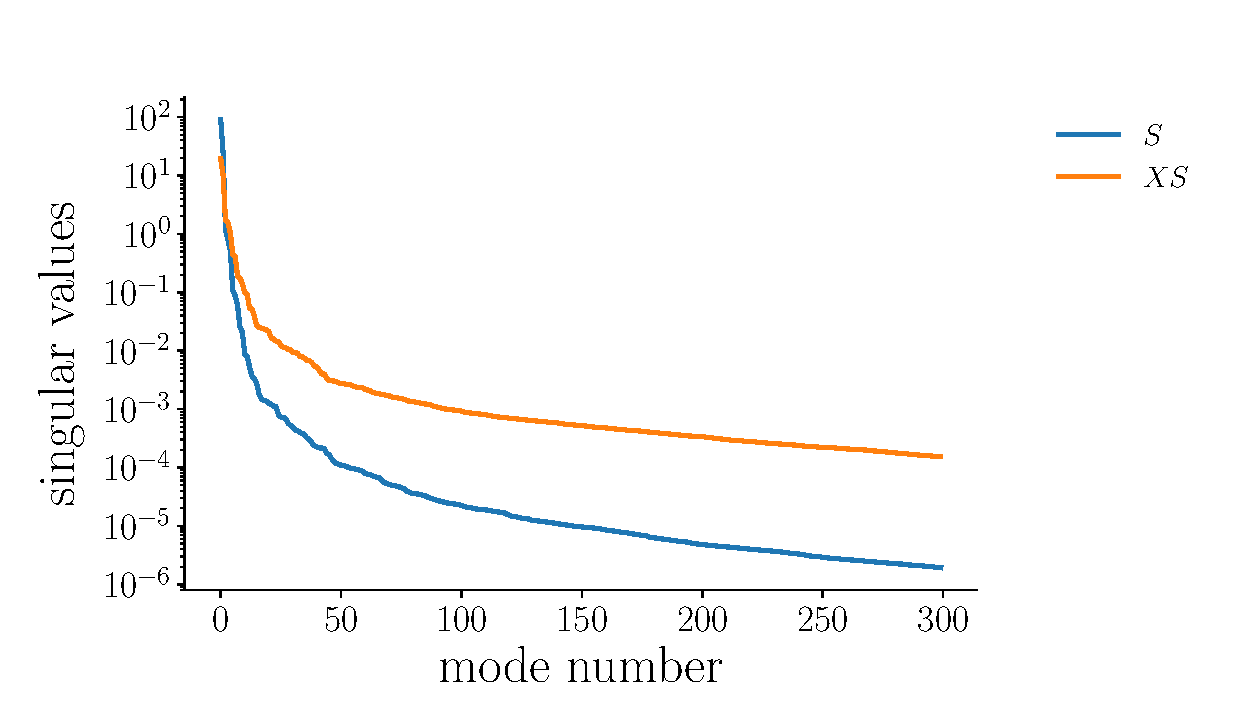
\includegraphics[width=0.45\textwidth]{./figs/beam/singulars} & 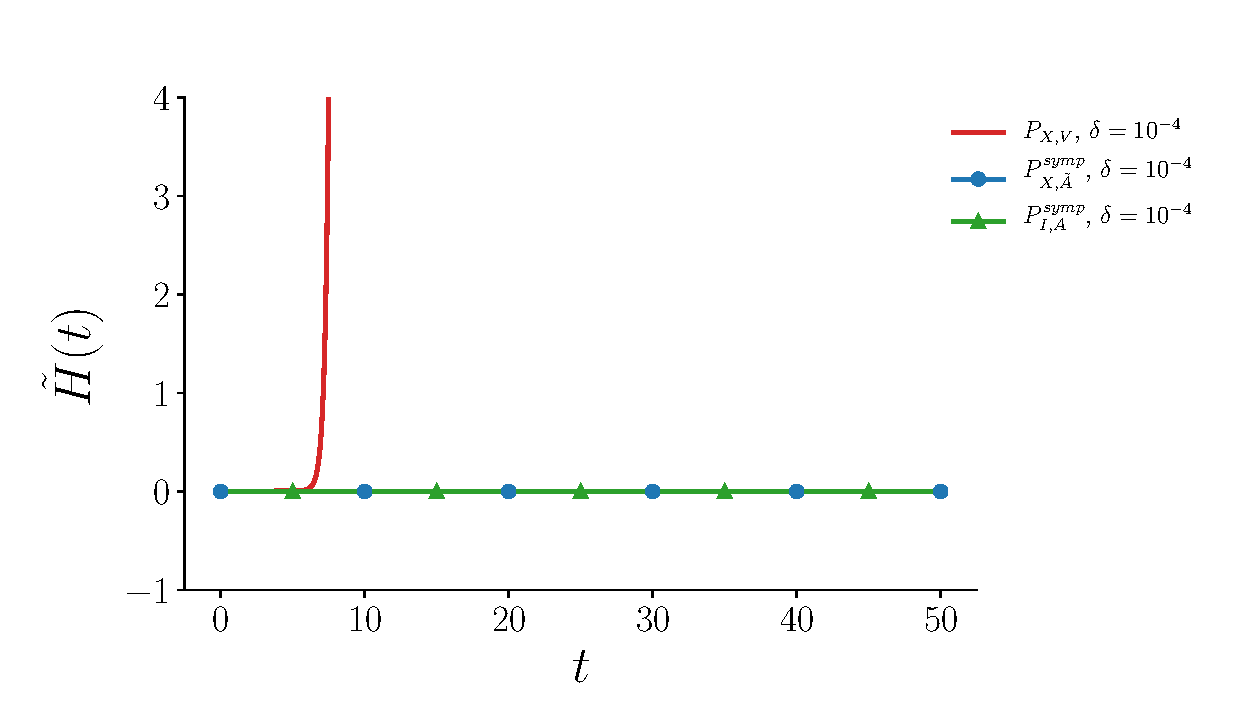
\includegraphics[width=0.45\textwidth]{./figs/beam/energy} \\
(a) & (b) \\
%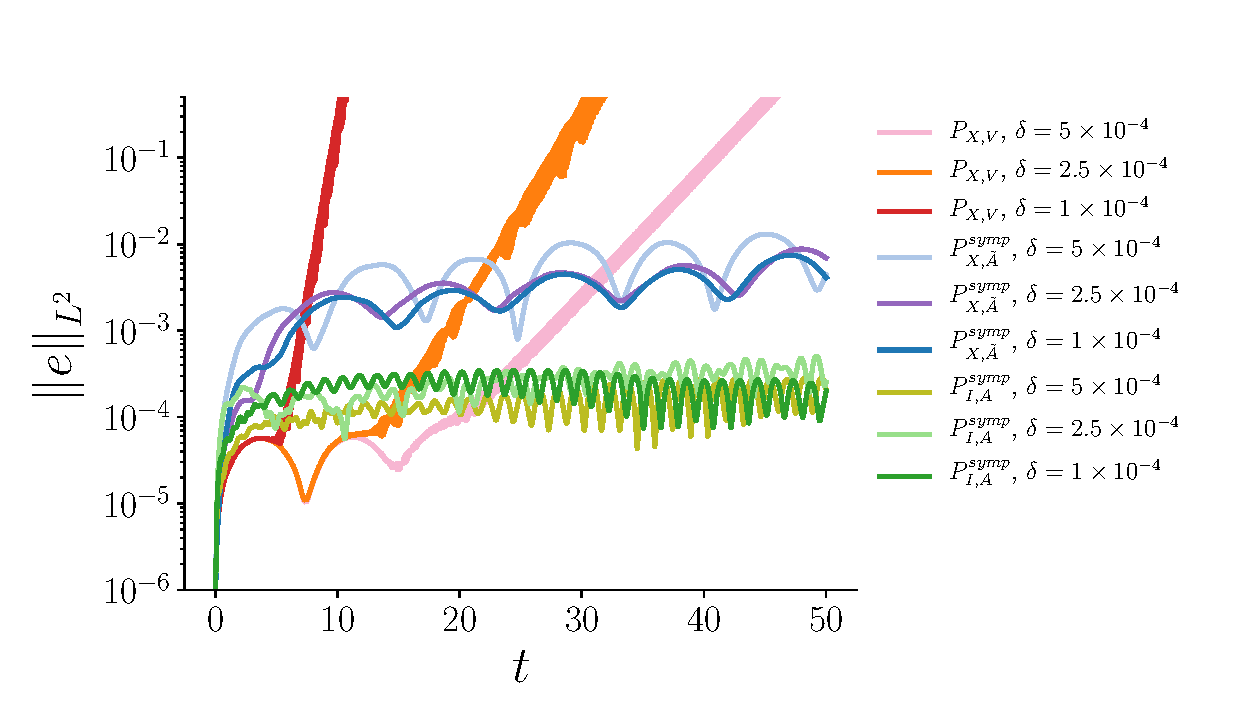
\includegraphics[width=0.45\textwidth]{./figs/beam/l2_norm} & 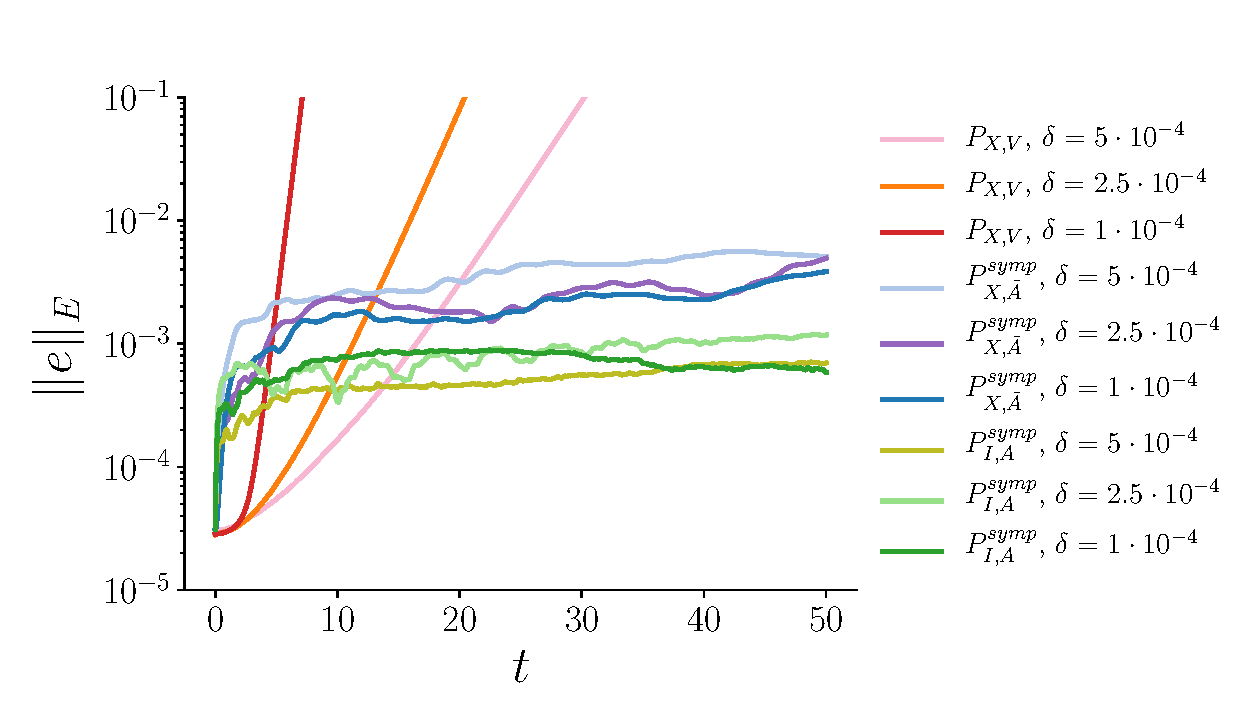
\includegraphics[width=0.45\textwidth]{./figs/beam/energy_norm} \\
\multicolumn{2}{c}{
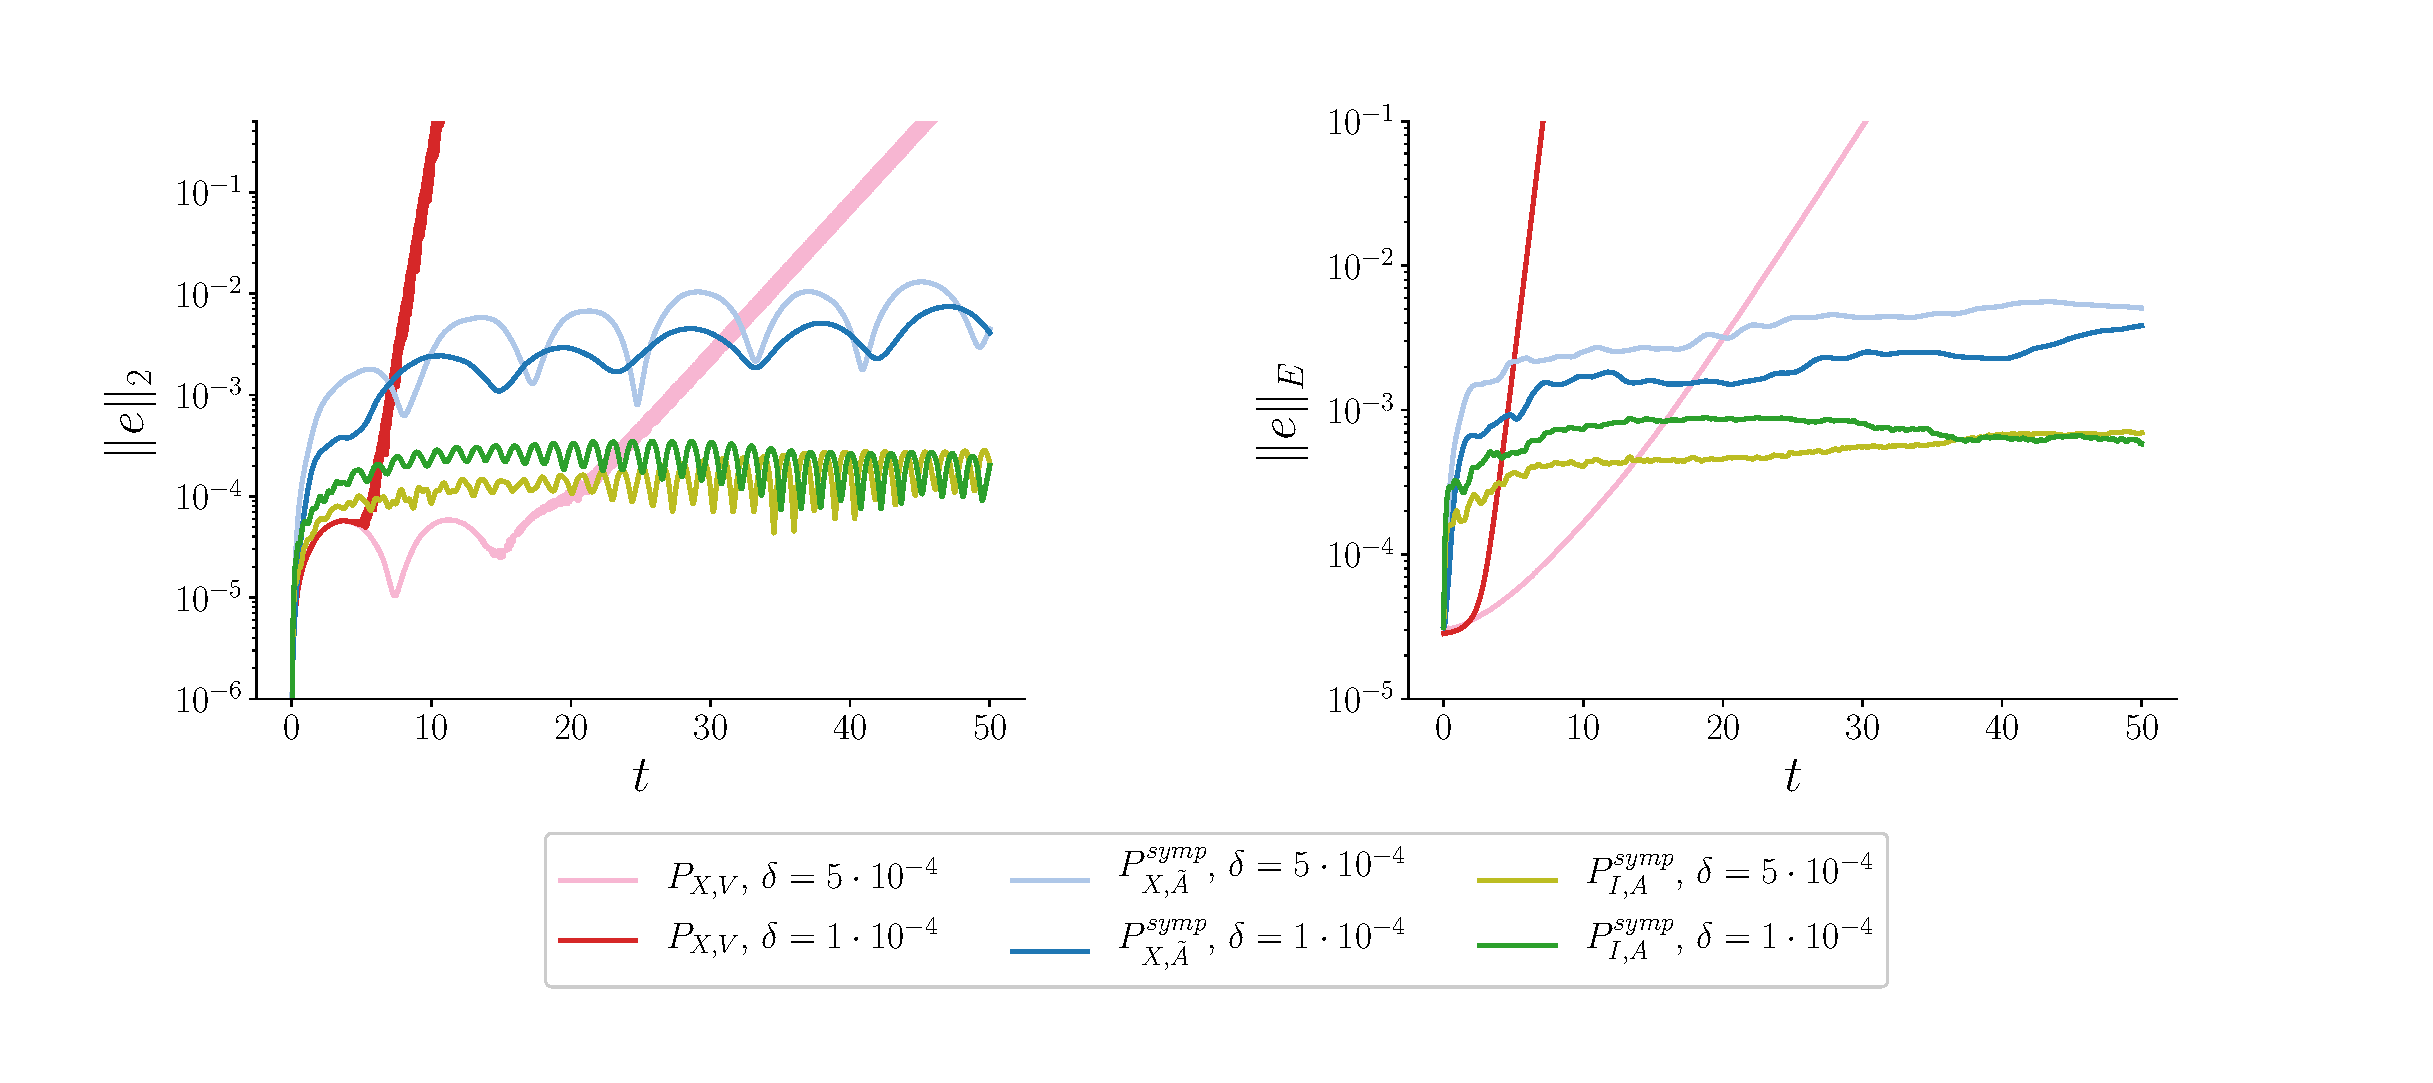
\includegraphics[width=0.96\textwidth]{./figs/beam/error_combined} }\\
(c) & (d) \\
\end{tabular}
\caption{Numerical results related to the beam equation. (a) the decay of the singular values. (b) conservation of the Hamiltonian. (c) error with respect to the 2-norm. (d) error with respect to the $X$-norm.}
\end{figure}

\Cref{fig:1}(a) shows the decay of the singular values of the temporal snapshots $S$ and $XS$, respectively. The difference in the decay indicates that the reduced systems constructed using $P_{I,A}^{\text{symp}}$ and $P_{X,\tilde A}^{\text{symp}}$ would have different sizes to achieve similar accuracy.

\Cref{fig:1}(b) shows the conservation of the Hamiltonian for the methods discussed above. This confirms that the symplectic methods preserve the Hamiltonian and the system energy. However, the Hamiltonian blows up for the reduced system constructed by the projection $P_{X,V}$.

\Cref{fig:1}(c) shows the $L^2$ error between the projected systems and the full order system, defined as
\begin{equation}
	\| e \|_{L^2} = \sqrt{(e,e)} \approx \sqrt{ (q - \hat q)^T M (q-\hat q) },
\end{equation}
where $e\in V$ is the error function and $\hat q \in \mathbb R^{2n}$ is an approximation for $q$. We notice that the reduced system obtained by the non-symplectic method is unstable and the reduced system, constructed using $P_{X,V}$, is more unstable as $k$ increases. On the other hand, the symplectic methods yield a stable reduced system. Although the system, constructed by the projection $P^{\text{symp}}_{X,\tilde A}$, is not based on the 2-norm projection, the error remains bounded with respect to the 2-norm. 

We define the energy norm $\| \cdot \|_E : V \to \mathbb R$ as
\begin{equation}
	\| (u,\dot u) \|_E = \sqrt{ a(u,u) + (\dot u , \dot u) } \approx \| z \|_X.
\end{equation}
\Cref{fig:1}(d) shows the MOR error with respect to the energy norm. We observe that the classical model reduction method based on the projection $P_{X,V}$ does not yield a stable reduced system. However, the symplectic methods provide a stable reduced system. We observe that the original symplectic approach also provides an accurate solution with respect to the energy norm. Nevertheless, the relation between the two norms depends on the problem set up and the choice of discretization \cite{DEPARIS20094359}.

\subsection{Elastic beam with cavity}  \label{sec:res.1.1}
In this section we investigate the performance of the proposed method on a two dimensional elastic beam that contains a cavity. In this case a nonuniform triangulated mesh is desirable to balance the computational cost of a FEM discretization with the numerical error around the cavity. \Cref{fig:0}(a) shows the nonuniform mesh used in this section.
System parameters are taken to be identical to those in \cref{sec:res.1}. Numerical parameters are summarized in the table below.
\vspace{0.5cm}
\begin{center}
\begin{tabular}{|l|l|}
\hline
cavity width & $l_c = 0.1$ \\
Time step-size & $\Delta t = 4\times 10^{-4}$ \\
Degrees of freedom & $2N_{h} = 744$ \\
\hline
\end{tabular}
\end{center}
\vspace{0.5cm}


\begin{figure} \label{fig:1.1}
\begin{tabular}{cc}
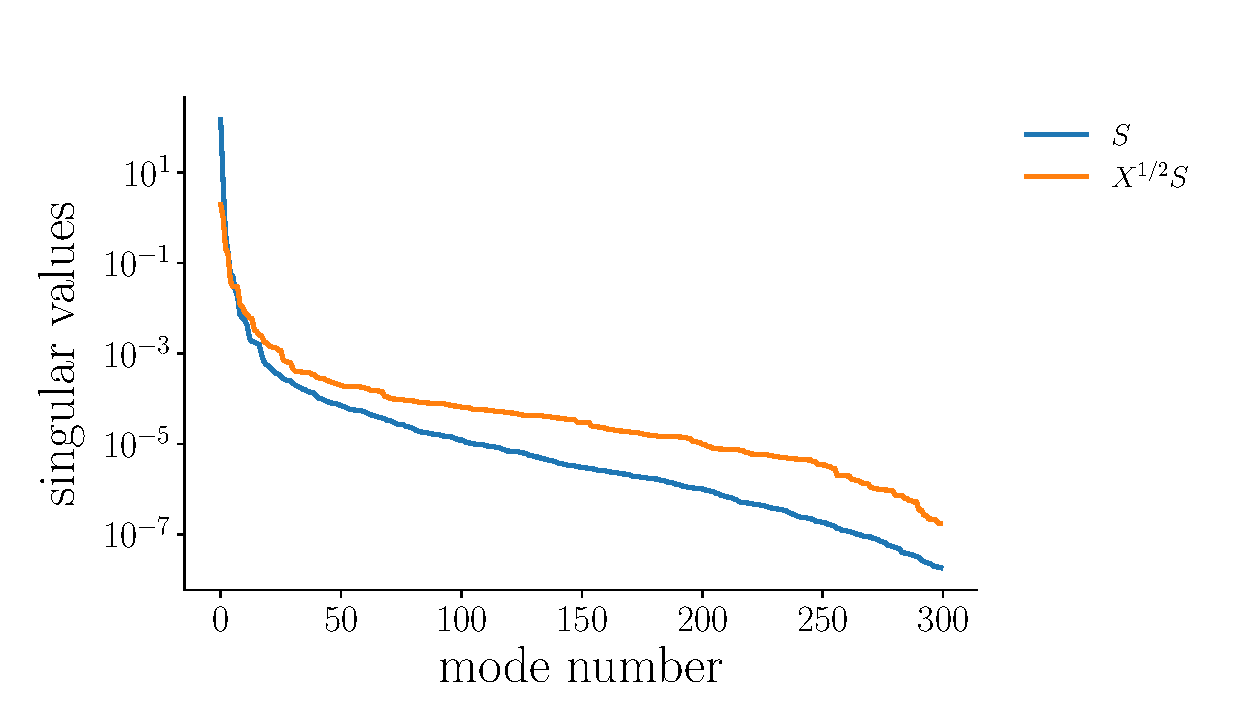
\includegraphics[width=0.45\textwidth]{./figs/beam_cracked/singulars} & 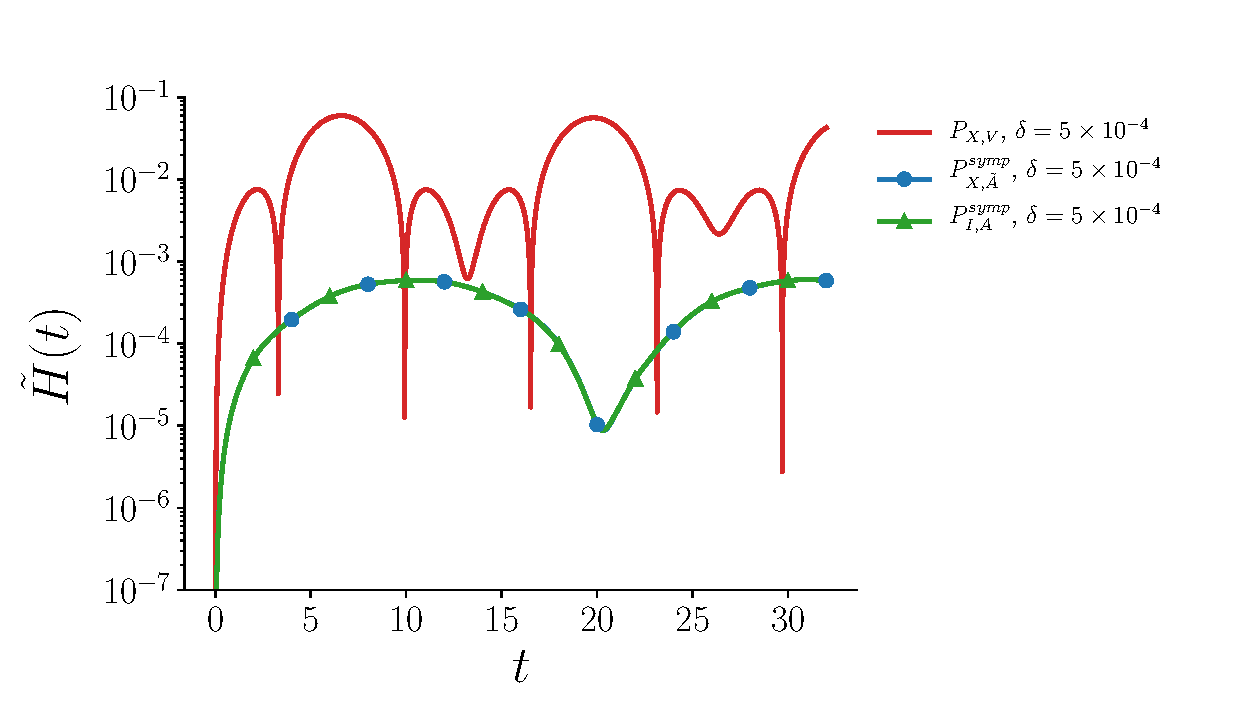
\includegraphics[width=0.45\textwidth]{./figs/beam_cracked/energy} \\
(a) & (b) \\
\multicolumn{2}{c}{
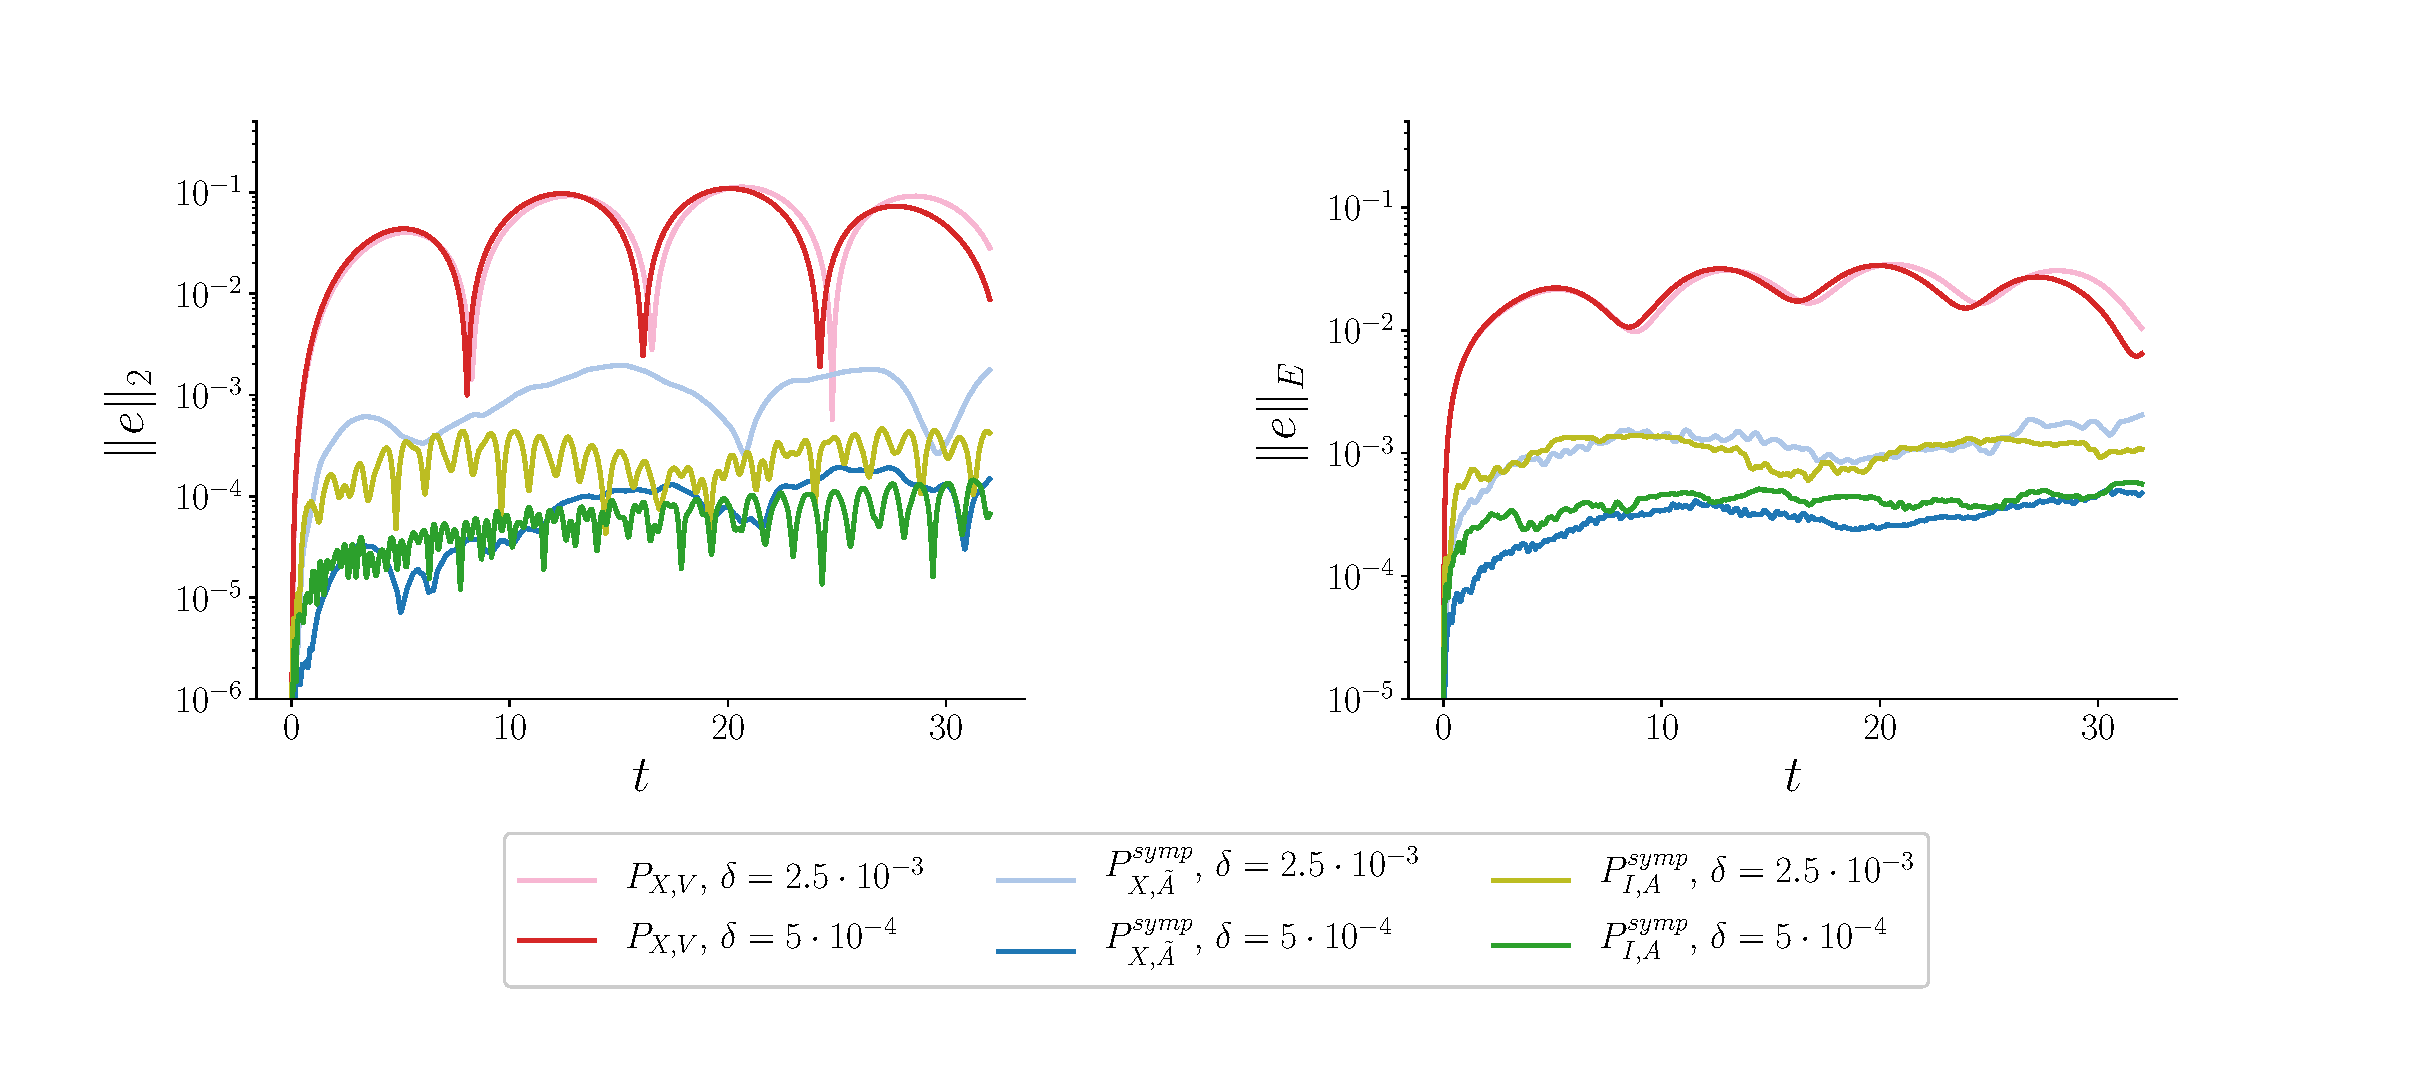
\includegraphics[width=0.96\textwidth]{./figs/beam_cracked/error_combined} }\\
(c) & (d) \\
\end{tabular}
\caption{Numerical results related to the beam with cavity. (a) the decay of the singular values. (b) conservation of the Hamiltonian. (c) error with respect to the 2-norm. (d) error with respect to the energy norm.}
\end{figure}

\Cref{fig:1.1}(a) shows the decay of the singular values for the snapshot matrix $S$ and $XS$. The divergence of the two curves indicates that to obtain the same accuracy in the reduced system, the basis constructed from $S$ and $XS$ would have different sizes.
Projection operators $P_{X,A}$, $P_{I,A}^{\text{symp}}$ and $P_{X,\tilde A}^{\text{symp}}$ are constructed according to the \cref{sec:mor.1,sec:mor.2,sec:mor.3}. The truncation error is set to $\delta = 2.5\times 10^{-3}$, 
$\delta = 1\times 10^{-3}$ and $\delta = 5\times 10^{-4}$ in \cref{alg:1,alg:2}

The 2-norm error and the error in the energy norm are presented in \Cref{fig:1.1}(c) and \Cref{fig:1.1}(d), respectively. We notice that although the non-symplectic method is bounded, it contains larger error compared to the symplectic methods. Moreover, we notice that the error generated by the symplectic methods is consistently reduced under basis enrichment. It is observed that in the energy norm, the projection $P_{X,\tilde A}^{\text{symp}}$ provides a more accurate solution (compare to \Cref{fig:1}). This is because on a nonuniform mesh, the weight matrix $X$ associates higher weights to the elements that are subject to larger error. Therefore, we expect the reduced system constructed with the projection $P_{X,\tilde A}^{\text{symp}}$ to outperform the one constructed with $P_{I,A}^{\text{symp}}$ on a highly nonuniform mesh.

\Cref{fig:1.1}(b) shows the error in the Hamiltonian. Comparing to \Cref{fig:1}, we notice that the energy norm helps with the boundedness of the non-symplectic method. However, the symplectic methods preserves the Hamiltonian at a higher accuracy

\subsection{The sine-Gordon equation} \label{sec:res.2}
The sine-Gordon equation arises in differential geometry and quantum physics \cite{Misumi2015}, as a nonlinear generalization of the linear wave equation of the form
\begin{equation} \label{eq:res.12}
\left\{
\begin{aligned}
	u_{t}(t,x) &= v, \quad x\in \Gamma,\\
	v_t(t,x) &= u_{xx} - \sin(u), \\
	u(t,0) &= 0, \\
	u(t,l) &= 2\pi.
\end{aligned}
\right.
\end{equation}
Here $\Gamma = [0,l]$ is a line segment and $u,v: \Gamma \to \mathbb R$ are scalar functions. The Hamiltonian associated with (\ref{eq:res.12}) is
\begin{equation} \label{eq:res.13}
	H(q,p) = \int_{\Gamma} \frac 1 2 p^2 + \frac 1 2 q_x^2 + 1 - \cos(q) \ dx.
\end{equation}
One can verify that $u_{t} = \delta_v H$ and $v_{t} = - \delta_u H$, where $\delta_v,\delta_u$ are standard variational derivatives. The sine-Gordon equation admits the soliton solution
\begin{equation} \label{eq:res.14}
	u(t,x) = 4 \text{arctan}\left( \exp \left( \pm \frac{x - x_0 - ct}{\sqrt{1-c^2}} \right) \right),
\end{equation}
where $x_0 \in \Gamma$ and the plus and minus signs correspond to the \emph{kink} and the \emph{anti-kink} solutions, respectively. Here $c$, $|c|<1$, is the arbitrary wave speed. We discretize the segment into $n$ equi-distant grid point $x_i = i\Delta x$, $i=1,\dots,n$. Furthermore, we use standard finite-differences schemes to discretize (\ref{eq:res.12}) and obtain
\begin{equation} \label{eq:res.15}
	\dot z = \mathbb J_{2n} L z + \mathbb J_{2n} g(z) + \mathbb J_{2n} c_b.
\end{equation}
Here $z = (q^T,p^T)^T$, $q(t) = (u(t,x_1),\dots,u(t,x_N))^T$, $p(t) = (v(t,x_1),\dots,v(t,x_N))^T$, $c_b$ is the term corresponding to the boundary conditions and
\begin{equation} \label{eq:res.16}
	L = 
	\begin{pmatrix}
		D_x^TD_x & 0_N \\
		0_N & I_n
	\end{pmatrix}, 
	\quad
	g(z) = 
	\begin{pmatrix}
	\sin(q) \\
	\vec 0
	\end{pmatrix},
\end{equation}
where $D_x$ is the standard matrix differentiation operator. We may take $X = L$ as the weight matrix associated to (\ref{eq:res.15}). The discrete Hamiltonian, takes the form
\begin{equation} \label{eq:res.17}
	H_{\Delta x} = \Delta x \cdot \frac 1 2 \| p \|^2_2 + \Delta x \cdot \| D_x q \|^2_2 + \sum_{i=1}^{n} \Delta x \cdot ( 1 - \cos(q_i) ).
\end{equation}
The system parameters are given as
\vspace{0.5cm}
\begin{center}
\begin{tabular}{|l|l|}
\hline
Domain length & $l = 50$ \\
No. grid points & $n = 500$ \\
Time step-size & $\Delta t = 0.01$ \\
Wave speed & $c=0.2$ \\
\hline
\end{tabular}
\end{center}
\vspace{0.5cm}
The midpoint scheme (\ref{eq:hamil.7}) is used to integrate (\ref{eq:res.12}) in time and generate the snapshot matrix $S$. Similar to the previous subsection, projection operators $P_{X,V}$, $P^{\text{symp}}_{I,A}$ and $P^{\text{symp}}_{X,\tilde A}$ are used to construct a reduced system. To accelerate the evaluation of the nonlinear term, the symplectic methods discussed in \cref{sec:mor.1,sec:mor.2} are coupled with the projection operators $P^{\text{symp}}_{I,A}$ and $P^{\text{symp}}_{X,A}$, respectively. Furthermore, the DEIM approximation is used for the efficient evaluation of the reduced system, obtained by the projection $P_{X,V}$. The midpoint rule is also used to integrate the reduced systems in time. \Cref{fig:2} shows the numerical results corresponding to the reduced models without approximating the nonlinearity, while the results corresponding to the accelerated evaluation of the nonlinear term are presented in \Cref{fig:3}.

\begin{figure} \label{fig:2}
\begin{tabular}{cc}
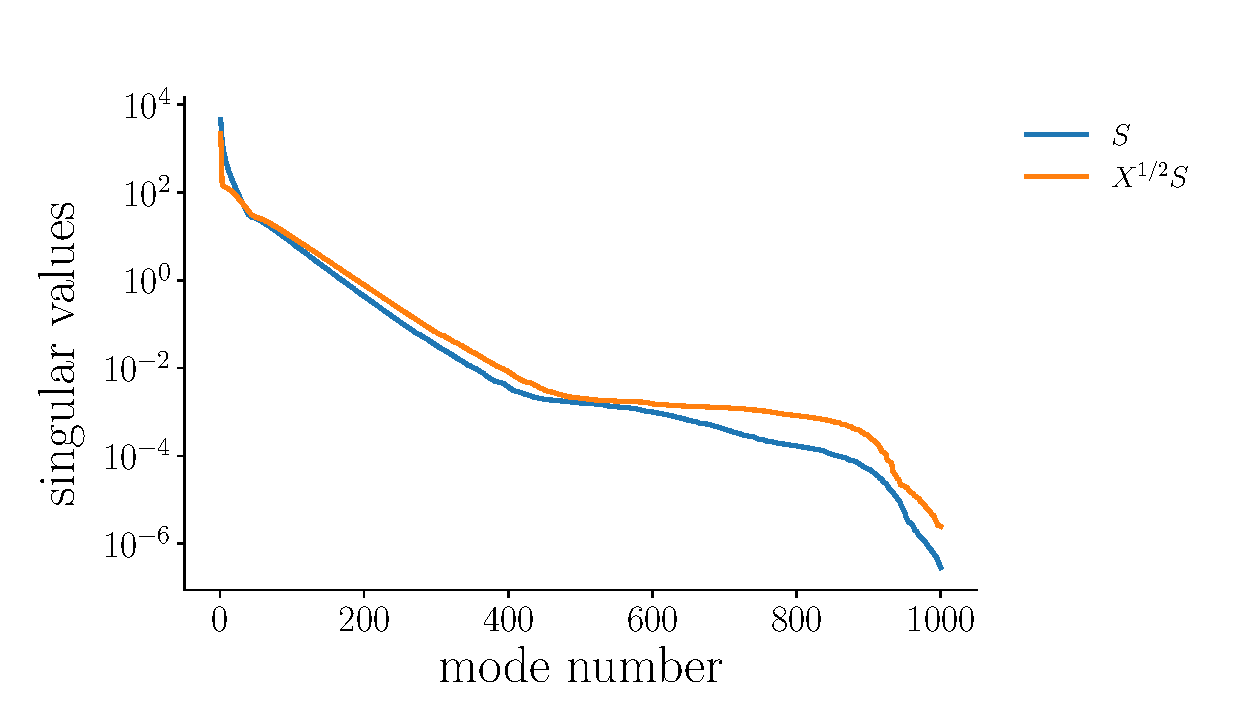
\includegraphics[width=0.45\textwidth]{./figs/sine/singulars} & 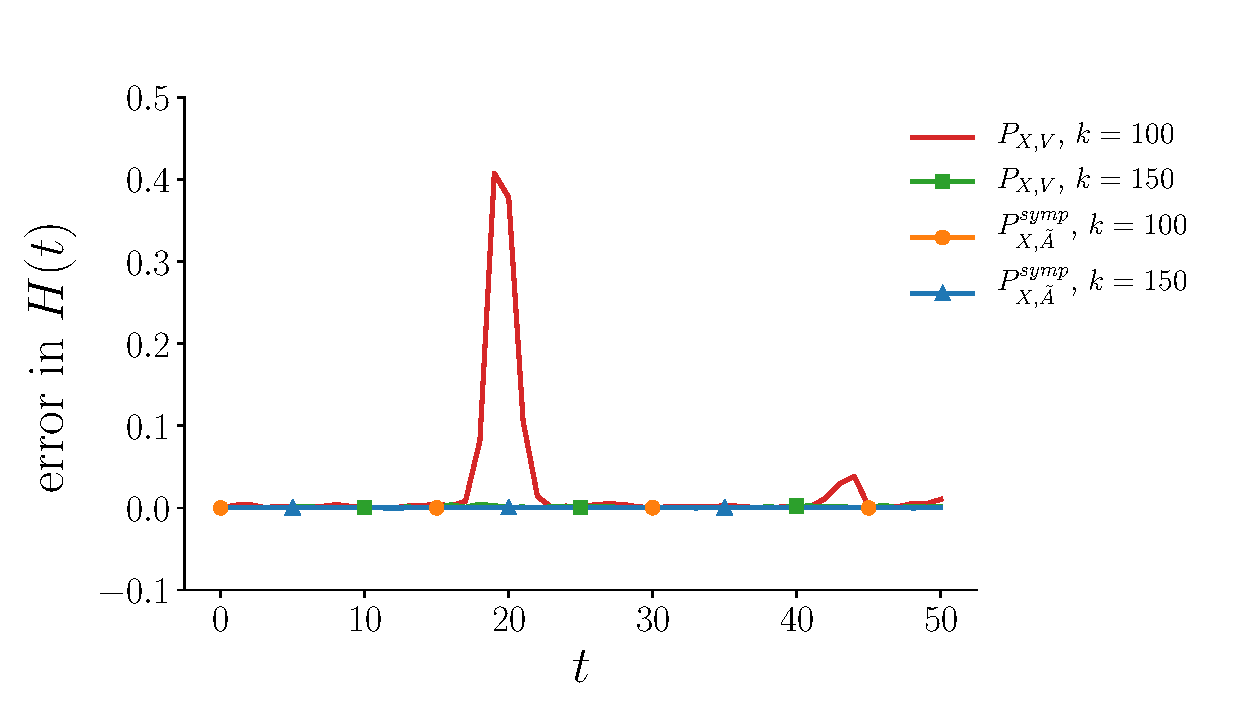
\includegraphics[width=0.45\textwidth]{./figs/sine/energy} \\
(a) & (b) \\
\multicolumn{2}{c}{
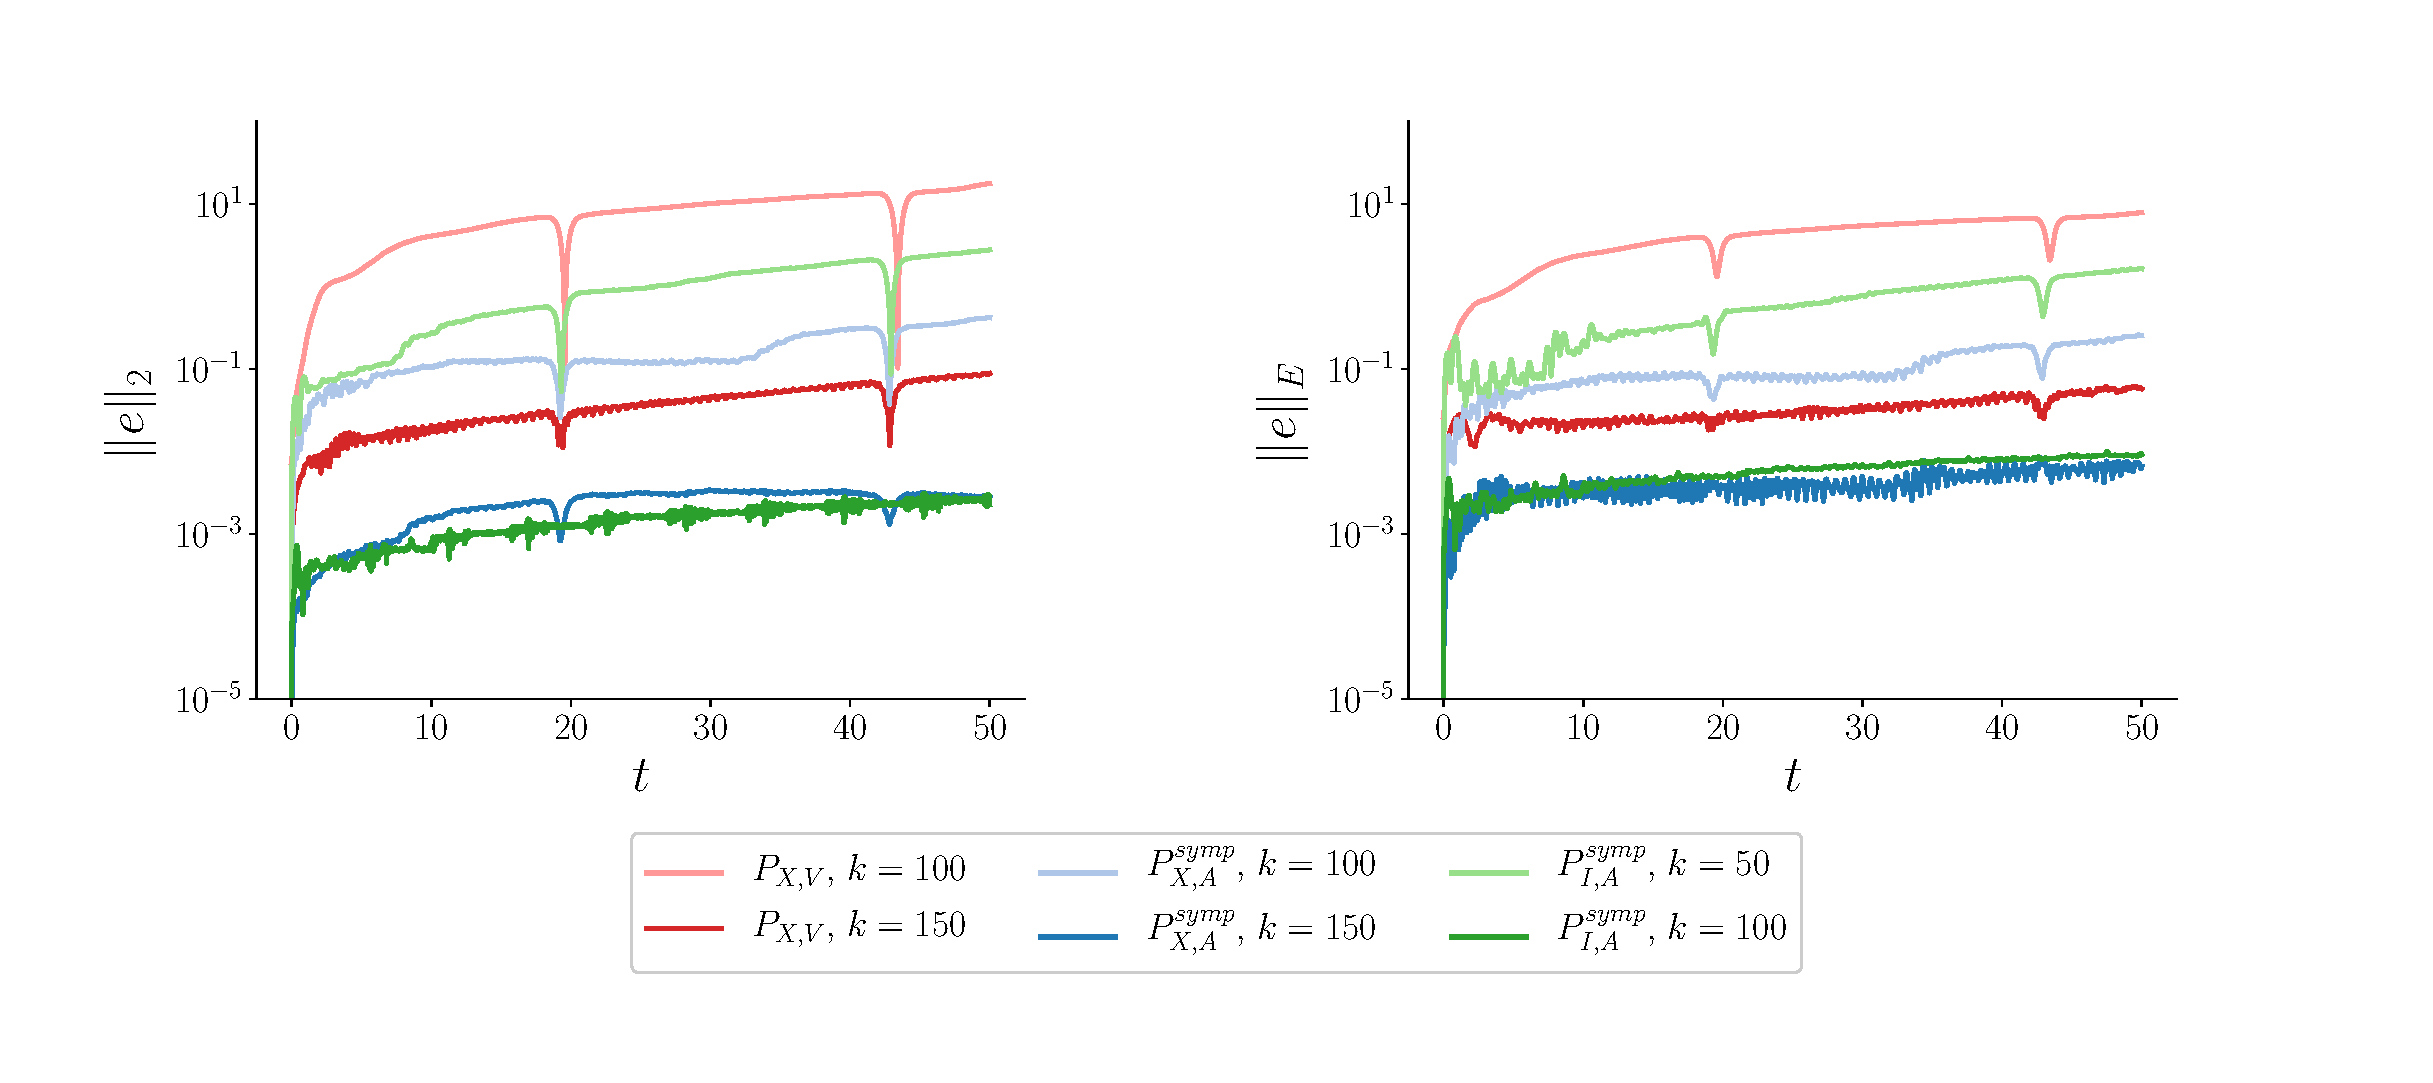
\includegraphics[width=0.96\textwidth]{./figs/sine/error_combined} }\\
(c) & (d) \\
\end{tabular}
\caption{Numerical results related to the sine-Gordon equation. (a) the decay of the singular values. (b) error in the Hamiltonian. (c) error with respect to the 2-norm. (d) error with respect to the energy norm.}
\end{figure}

\Cref{fig:2}(a) shows the decay of the singular values of matrices $S$ and $XS$. As in the previous section, we observe a saturation in the decay of the singular values of $XS$ compared to the singular values of $S$. This indicates that the reduced basis, based on a weighted inner product, should be chosen to be larger to provide an accuracy similar to based on the Euclidean inner product. Put differently, unweighted reduced bases, when compared to the weighted ones, may be highly inaccurate in reproducing underlying physical properties of the system.

\Cref{fig:2}(b) displays the error in the Hamiltonian. It is observed again that the symplectic approaches conserve the Hamiltonian. However, the classical approaches do not necessarily conserve the Hamiltonian. We point out that using the projection operator $P_{X,V}$ ensures the boundedness of the Hamiltonian. The contrary is observed when we apply the POD with respect to the Euclidean inner-product, i.e. applying the projection operator $P_{I,V}$. This can be seen in the results presented in \cite{doi:10.1137/140978922}, where the unboundedness of the Hamiltonian is observed when $P_{I,V}$ is applied to the sine-Gordon equation. Nevertheless, only the symplectic model reduction consistently preserves the Hamiltonian.

\Cref{fig:2}(c) shows the error with respect to the Euclidean inner-product between the solution of the projected systems and the original system. The behavior of the solution is investigated for $k=100$, $k=125$ and $k=150$. We observe that all systems which are projected with respect to the $X$-norm are bounded. As the results in \cite{doi:10.1137/140978922} suggest, the Euclidean inner-product does not necessarily yield a bounded reduced system. Moreover, we notice that the symplectic projection $P^{\text{symp}}_{X,\tilde A}$ results in a substantially more accurate reduced system compared to the reduced system yielded from $P_{X,V}$. This is because the overall behavior of the original system is translated correctly to the reduced system constructed with the symplectic projection.

The error with respect to the $X$-norm between the solution of the original system and the projected systems is presented in \Cref{fig:2}(d). We see that the behavior of the $X$-norm error is similar to the Euclidean norm, however the growth of the error is slower for methods based on a weighted inner product. Note that the connection between the error in the Euclidean norm and the $X$-norm is problem and discretization dependent. We also observed that symplectic methods are substantially more accurate.

\begin{figure} \label{fig:3}
\begin{tabular}{cc}
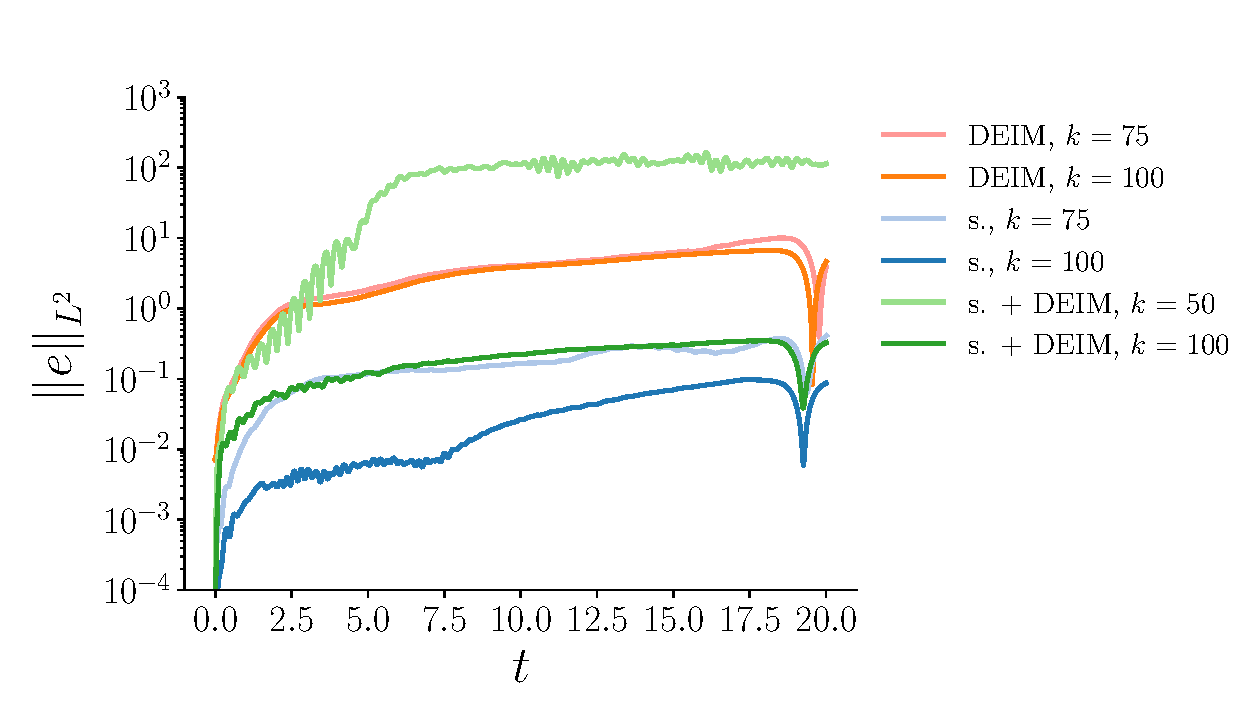
\includegraphics[width=0.45\textwidth]{./figs/sine/nonlinear/l2} & 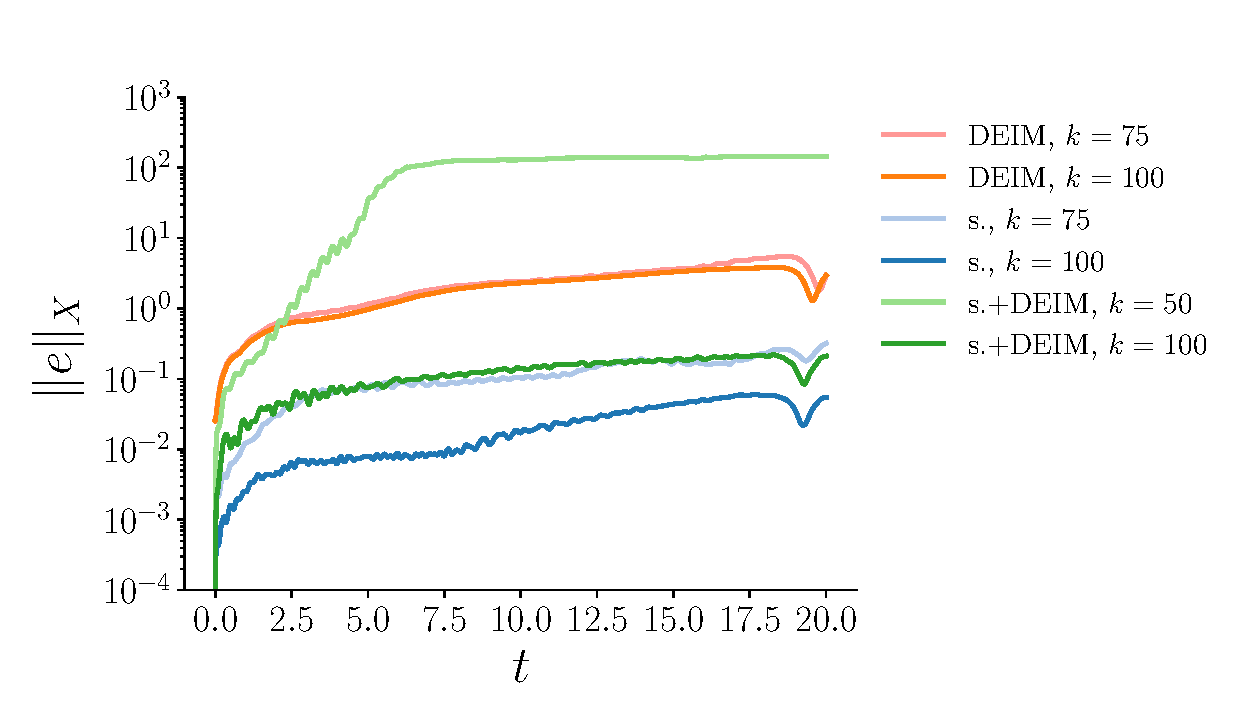
\includegraphics[width=0.45\textwidth]{./figs/sine/nonlinear/energy_norm} \\
(a) & (b) \\
\multicolumn{2}{c}{
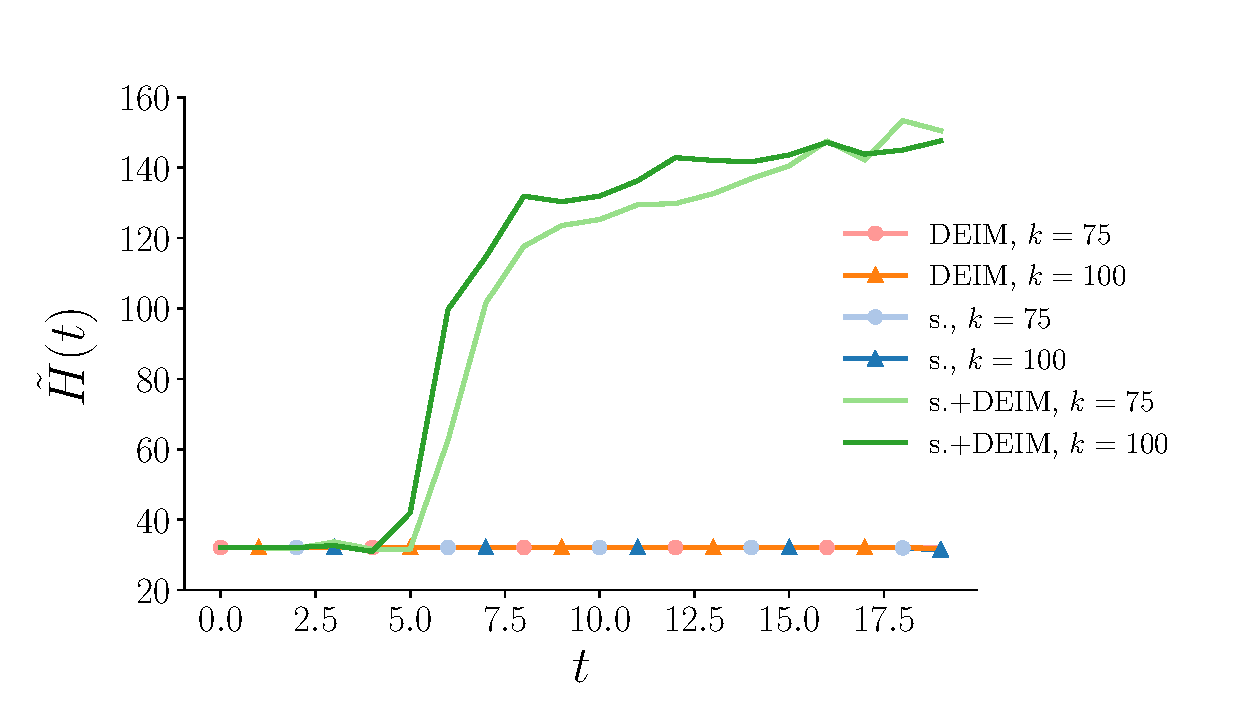
\includegraphics[width=0.45\textwidth]{./figs/sine/nonlinear/energy}
} \\
\multicolumn{2}{c}{(c)} \\
\end{tabular}
\caption{Numerical results related to the sine-Gordon equation with efficient evaluation of the nonlinear terms. Here, ``DEIM'' indicates classical model reduction with the DEIM, ``s.+DEIM'' indicates symplectic model reduction with the DEIM and ``s.'' indicates symplectic model reduction with symplectic treatment of the nonlinear term. (a) error with respect to the Euclidean norm. (b) error with respect to the $X$-norm. (c) error in the Hamiltonian. }
\end{figure}

\Cref{fig:3} shows the performance of the different model reduction methods, when an efficient method is adopted in evaluating the nonlinear term in (\ref{eq:res.15}). This figure compares the symplectic approaches against non-symplectic methods. For all simulations, the size of the reduced basis for (\ref{eq:res.15}) is chosen to be $k=100$. The size of the basis of the nonlinear term is then taken as $k_n=75$ and $k_n=100$. For symplectic methods, a basis for the nonlinear term is constructed according to \Cref{alg:3}, whereas for non-symplectic methods, the DEIM is applied. Note that for symplectic methods, the basis for the nonlinear term is added to the symplectic basis $A$. This means that the size of the reduced system is larger compared to the classical approach.

\Cref{fig:3}(a) and \Cref{fig:3}(b) show the error with respect to the Euclidean norm and the $X$-norm between the solution of the projected systems compared to the solution of the original system, respectively. We observe that all solutions are bounded and the behavior of the error in the Euclidean norm and the $X$-norm is similar. We observe that enriching the DEIM basis does not increase the overall accuracy of the system projected using $P_{X,V}$. Furthermore, applying the DEIM to a symplectic reduced system also destroys the symplectic nature of the reduced system, as suggested in \cref{sec:normmor.3}. Therefore, it is essential to adopt a symplectic approach to reduce the complexity of the evaluation of the nonlinear terms. We observe that the symplectic method presented in \cref{sec:normmor.3} provides not only an accurate approximation of the nonlinear term, but also preserves the symplectic structure of the reduced system. Moreover, enriching such a basis consistently increases the accuracy of the solution, as suggested in \Cref{fig:3}(a) and \Cref{fig:3}(b).

\Cref{fig:3}(b) shows the conservation of the Hamiltonian for different methods. It is again visible that applying the DEIM to a symplectic reduced system destroys the Hamiltonian structure, therefore the Hamiltonian is not preserved.


